% Options for packages loaded elsewhere
\PassOptionsToPackage{unicode}{hyperref}
\PassOptionsToPackage{hyphens}{url}
\PassOptionsToPackage{dvipsnames,svgnames,x11names}{xcolor}
%
\documentclass[
  rmp,
  amsmath,
  amssymb,
  preprint]{revtex4-2}

\usepackage{amsmath,amssymb}
\usepackage{iftex}
\ifPDFTeX
  \usepackage[T1]{fontenc}
  \usepackage[utf8]{inputenc}
  \usepackage{textcomp} % provide euro and other symbols
\else % if luatex or xetex
  \usepackage{unicode-math}
  \defaultfontfeatures{Scale=MatchLowercase}
  \defaultfontfeatures[\rmfamily]{Ligatures=TeX,Scale=1}
\fi
\usepackage{lmodern}
\ifPDFTeX\else  
    % xetex/luatex font selection
\fi
% Use upquote if available, for straight quotes in verbatim environments
\IfFileExists{upquote.sty}{\usepackage{upquote}}{}
\IfFileExists{microtype.sty}{% use microtype if available
  \usepackage[]{microtype}
  \UseMicrotypeSet[protrusion]{basicmath} % disable protrusion for tt fonts
}{}
\makeatletter
\@ifundefined{KOMAClassName}{% if non-KOMA class
  \IfFileExists{parskip.sty}{%
    \usepackage{parskip}
  }{% else
    \setlength{\parindent}{0pt}
    \setlength{\parskip}{6pt plus 2pt minus 1pt}}
}{% if KOMA class
  \KOMAoptions{parskip=half}}
\makeatother
\usepackage{xcolor}
\setlength{\emergencystretch}{3em} % prevent overfull lines
\setcounter{secnumdepth}{5}
% Make \paragraph and \subparagraph free-standing
\ifx\paragraph\undefined\else
  \let\oldparagraph\paragraph
  \renewcommand{\paragraph}[1]{\oldparagraph{#1}\mbox{}}
\fi
\ifx\subparagraph\undefined\else
  \let\oldsubparagraph\subparagraph
  \renewcommand{\subparagraph}[1]{\oldsubparagraph{#1}\mbox{}}
\fi


\providecommand{\tightlist}{%
  \setlength{\itemsep}{0pt}\setlength{\parskip}{0pt}}\usepackage{caption}
% \usepackage{longtable,booktabs,array}
\usepackage{calc} % for calculating minipage widths
% Correct order of tables after \paragraph or \subparagraph
\usepackage{etoolbox}
\makeatletter
\patchcmd\longtable{\par}{\if@noskipsec\mbox{}\fi\par}{}{}
\makeatother
% Allow footnotes in longtable head/foot
\IfFileExists{footnotehyper.sty}{\usepackage{footnotehyper}}{\usepackage{footnote}}
\makesavenoteenv{longtable}
\usepackage{graphicx}
\makeatletter
\def\maxwidth{\ifdim\Gin@nat@width>\linewidth\linewidth\else\Gin@nat@width\fi}
\def\maxheight{\ifdim\Gin@nat@height>\textheight\textheight\else\Gin@nat@height\fi}
\makeatother
% Scale images if necessary, so that they will not overflow the page
% margins by default, and it is still possible to overwrite the defaults
% using explicit options in \includegraphics[width, height, ...]{}
\setkeys{Gin}{width=\maxwidth,height=\maxheight,keepaspectratio}
% Set default figure placement to htbp
\makeatletter
\def\fps@figure{htbp}
\makeatother
\newlength{\cslhangindent}
\setlength{\cslhangindent}{1.5em}
\newlength{\csllabelwidth}
\setlength{\csllabelwidth}{3em}
\newlength{\cslentryspacingunit} % times entry-spacing
\setlength{\cslentryspacingunit}{\parskip}
\newenvironment{CSLReferences}[2] % #1 hanging-ident, #2 entry spacing
 {% don't indent paragraphs
  \setlength{\parindent}{0pt}
  % turn on hanging indent if param 1 is 1
  \ifodd #1
  \let\oldpar\par
  \def\par{\hangindent=\cslhangindent\oldpar}
  \fi
  % set entry spacing
  \setlength{\parskip}{#2\cslentryspacingunit}
 }%
 {}
\usepackage{calc}
\newcommand{\CSLBlock}[1]{#1\hfill\break}
\newcommand{\CSLLeftMargin}[1]{\parbox[t]{\csllabelwidth}{#1}}
\newcommand{\CSLRightInline}[1]{\parbox[t]{\linewidth - \csllabelwidth}{#1}\break}
\newcommand{\CSLIndent}[1]{\hspace{\cslhangindent}#1}

% \usepackage{float}
% \makeatletter
% \let\oldlt\longtable
% \let\endoldlt\endlongtable
% \def\longtable{\@ifnextchar[\longtable@i \longtable@ii}
% \def\longtable@i[#1]{\begin{figure}[H]
% \onecolumn
% \begin{minipage}{0.5\textwidth}
% \oldlt[#1]
% }
% \def\longtable@ii{\begin{figure}[H]
% \onecolumn
% \begin{minipage}{0.5\textwidth}
% \oldlt
% }
% \def\endlongtable{\endoldlt
% \end{minipage}
% \twocolumn
% \end{figure}}
% \makeatother
\makeatletter
\makeatother
\makeatletter
\makeatother
\makeatletter
\@ifpackageloaded{caption}{}{\usepackage{caption}}
\AtBeginDocument{%
\ifdefined\contentsname
  \renewcommand*\contentsname{Table of contents}
\else
  \newcommand\contentsname{Table of contents}
\fi
\ifdefined\listfigurename
  \renewcommand*\listfigurename{List of Figures}
\else
  \newcommand\listfigurename{List of Figures}
\fi
\ifdefined\listtablename
  \renewcommand*\listtablename{List of Tables}
\else
  \newcommand\listtablename{List of Tables}
\fi
\ifdefined\figurename
  \renewcommand*\figurename{Figure}
\else
  \newcommand\figurename{Figure}
\fi
\ifdefined\tablename
  \renewcommand*\tablename{Table}
\else
  \newcommand\tablename{Table}
\fi
}
\@ifpackageloaded{float}{}{\usepackage{float}}
\floatstyle{ruled}
\@ifundefined{c@chapter}{\newfloat{codelisting}{h}{lop}}{\newfloat{codelisting}{h}{lop}[chapter]}
\floatname{codelisting}{Listing}
\newcommand*\listoflistings{\listof{codelisting}{List of Listings}}
\makeatother
\makeatletter
\@ifpackageloaded{caption}{}{\usepackage{caption}}
\@ifpackageloaded{subcaption}{}{\usepackage{subcaption}}
\makeatother
\makeatletter
\@ifpackageloaded{tcolorbox}{}{\usepackage[skins,breakable]{tcolorbox}}
\makeatother
\makeatletter
\@ifundefined{shadecolor}{\definecolor{shadecolor}{rgb}{.97, .97, .97}}
\makeatother
\makeatletter
\makeatother
\makeatletter
\makeatother
\ifLuaTeX
  \usepackage{selnolig}  % disable illegal ligatures
\fi
\IfFileExists{bookmark.sty}{\usepackage{bookmark}}{\usepackage{hyperref}}
\IfFileExists{xurl.sty}{\usepackage{xurl}}{} % add URL line breaks if available
\urlstyle{same} % disable monospaced font for URLs
\hypersetup{
  pdftitle={Possible Periodictity of Two Fast Radio Bursts (FRB) Repeaters with Limited Detections: FRB20190915D and FRB20191106C},
  colorlinks=true,
  linkcolor={blue},
  filecolor={Maroon},
  citecolor={Blue},
  urlcolor={Blue},
  pdfcreator={LaTeX via pandoc}}

\title{Possible Periodictity of Two Fast Radio Bursts (FRB) Repeaters
with Limited Detections: FRB20190915D and FRB20191106C}
\date{}

\begin{document}
\begin{abstract}
    Fast radio burst (FRB) is a class of transients characterized by its
    miliseconds scale duration with a relatively high dispersion
    measure. Some of them show repetition and among those, only some of
    them seem to repeat regularly. This paper tries to characterize the
    periodicity of FRBs whose repetition seems to be limited within a
    certain timeframe -- FRB20190915D and FRB20191106C as the chosen
    examples -- from a 3 year dataset provided by the CHIME/FRB 2023
    Catalog. This paper found that the periodicity can be characterized
    with more than 50\% certainty despite the limited samples given that
    the waiting time is bimodally distributed.
\end{abstract}
\author{Murthadza AznamZamri Zainal AbidinNorsiah HashimMuhammad Hassan
Zakie YussoffMatdhesh Kummar Jayaganthan}
\maketitle
\ifdefined\Shaded\renewenvironment{Shaded}{\begin{tcolorbox}[frame hidden, boxrule=0pt, sharp corners, breakable, borderline west={3pt}{0pt}{shadecolor}, enhanced, interior hidden]}{\end{tcolorbox}}\fi

\hypertarget{introduction}{%
\section{Introduction}\label{introduction}}

Fast Radio Burst (FRB) is a class of transients first discovered by
Lorimer et al. (2007) with currently unknown origin. It is characterized
as a radio pulse with durations in the order of milliseconds and a
relatively high dispersion measure. Its high dispersion measure suggests
an extragalactic origin consistent with observation of identified hosts
such as in Bannister et al. (2019), Chatterjee et al. (2017), and Ravi
et al. (2019).

With increasing interests in FRBs, progress have been made in detections
(especially with the commisioning of the CHIME/FRB telescope (The
CHIME/FRB Collaboration et al. 2018) and in the future, BURSTT (Lin et
al. 2022)), theoretical models (a list of theories can be found in
Platts et al. (2019)), and analyses (especially on regularly repeating
bursts such as FRB20121102A and FRB20180916B). For an in-depth review of
the growth of FRB research, readers are suggested to read Petroff,
Hessels, and Lorimer (2019) and their follow-up review Petroff, Hessels,
and Lorimer (2022).

Currently, FRBs can be categorized as repeating or non-repeating. The
population seem to favor non-repeating FRBs over repeating FRBs as The
CHIME/FRB Collaboration et al. (2018) reports on 18 (3.7\%) repeating
sources are among 492 FRB sources detected \footnote{\url{https://www.chime-frb.ca/catalog}}.
A recent paper (Andersen et al. 2023) estimates that repeating sources
constitutes about 2.6\% of known FRBs. However, it is important to note
that there is no guarantee that one-off FRBs will not repeat. Following
this assumption, the term `apparently non-repeating FRB' have been used
in various papers, such as in Cui, Zhang, Wang, Zhang, Li, Peng, Zhu,
Wang, et al. (2021), Cui, Zhang, Wang, Zhang, Li, Peng, Zhu, Strom, et
al. (2021), and Katz (2022).

Multiple statistical analyses seem to support the idea that they are
truly two different population of FRBs with consistent differences
between repeating and non-repeating FRB in various properties (Cui,
Zhang, Wang, Zhang, Li, Peng, Zhu, Wang, et al. 2021; Chen et al. 2022;
Zhang et al. 2022). This consistency does not prevent some authors in
assuming that a small part of the non-repeating FRBs might repeat in the
future dubbed as `potentially repeating' or `repeater candidates', as
was done by Bo Han Chen et al. (2021), Luo, Zhu-Ge, and Zhang (2022),
Zhu-Ge, Luo, and Zhang (2022), and Pleunis et al. (2021).

Regularly repeating FRBs such as FRB20121102A and FRB20180916B are rare.
Most of the repeaters currently identified has a limited sample which
makes it hard to study its individual property. As such, many repeaters
are understudied as its low number of samples provide limited certainty.
This paper tries to study the property of individual sources with
limited samples.

Since periodicity generally requires many data points, this paper
examines whether it is possible to determine the periodicity of a source
with at least 50\% confidence using samples with more than 3 and less
than 20 event counts. If so, what are the criteria to differentiate
between determinable and non-determinable periodicity? Having this
criteria can help anticipate new detections.

\hypertarget{methodology}{%
\section{Methodology}\label{methodology}}

This paper will examine the periodicity of FRB20190915D (10 detections)
and FRB20191106C (7 detections) from the CHIME/FRB Catalog
2023\footnote{\url{https://www.chime-frb.ca/repeater_catalog}} (Andersen
et al. 2023). This paper will also include FRB20180916B (77 detections)
from CHIME/FRB Catalog 1 \footnote{\url{https://www.chime-frb.ca/catalog}}
(The CHIME/FRB Collaboration et al. 2021) to compare the validity of
methods since its periodicity value is well quantified to be around 16
days (The CHIME/FRB Collaboration et al. 2020; Sand et al. 2023).

\hypertarget{periodogram}{%
\subsection{Periodogram}\label{periodogram}}

A periodogram is a function of cost versus periods which quantifies the
strength of the fit between the given period and the time series data.
The cost function depends on the method of choice. The best period is
chosen based on the period with the maximum or minimum cost. While most
periodogram methods choose the best period via the maximum cost, the
phase dispersion minimization method chooses the minimum cost.
VanderPlas (2018) includes four types of periodograms: (1) Fourier
Method, based on Fourier transforms; (2) Phase-Folding Method, which
calculates cost by trying to fold phases at multiple trial periods; (3)
Least-Square Method, which fits a model time series; and (4) Bayesian
Approaches, which applies Bayesian probability to the problem.

\hypertarget{method-lombscargle-periodogram}{%
\subsubsection{Method: Lomb--Scargle
Periodogram}\label{method-lombscargle-periodogram}}

The Lomb--Scargle periodogram Scargle (1982) is the most commonly used
in astronomy. The cost function for this periodogram is the Fourier
power which is to be maximized. As such, it is a periodogram based on
Fourier transform but it can also be approached as a least square
optimization (VanderPlas 2018). The widespread use of this method
warrants its place in the \texttt{astropy} package\footnote{\url{https://docs.astropy.org/en/stable/api/astropy.timeseries.LombScargle.html}},
an astronomy package for the Python programming language.

\hypertarget{method-duty-cycle}{%
\subsubsection{Method: Duty Cycle}\label{method-duty-cycle}}

The Duty Cycle method is a phase--folding periodogram which measures the
trial period with the longest continuous inactivity per cycle of a given
FRB. This method was introduced by Rajwade et al. (2020) to measure the
periodicity of FRB20121102A because of the nature of repeaters to be
active within a certain period per cycle. A duty cycle of 56\% means
that there is a continuous inactivity for 44\% of the cycle.

\hypertarget{method-phase-dispersion-minimization}{%
\subsubsection{Method: Phase Dispersion
Minimization}\label{method-phase-dispersion-minimization}}

Phase Dispersion Minimization (PDM) is a phase--folding method to
determine the periodicity of non--sinusoidal time variation introduced
by Stellingwerf (1978). This method computes the variances,
\texttt{theta}, of the data with respect to mean light curve at each
trial periods and minimizes it. It is suitable for small dataset with
irregularly sampled observations, such as the repeaters sampled in the
CHIME/FRB 2023 Catalog. This paper will use the Python wrapper of this
algorithm written in C using the \texttt{py-pdm}\footnote{\url{https://github.com/ckm3/Py-PDM}}
package.

\hypertarget{parameter-frequency-grid}{%
\subsubsection{Parameter: Frequency
Grid}\label{parameter-frequency-grid}}

For this study, we chose a frequency grid of \(f_\text{max}\) = (3
days)\textsuperscript{-1} to
\(f_\text{min} = 0.5 * ( T_\text{obs}\, \text{days})^{-1}\), where
\(T_\text{obs}\) is the length of observation (1,007 days). The maximum
frequency is chosen such that if the period of FRBs is less than 3 days,
we would see it much more often at a daily or bidaily rate. On the other
hand, the minimum frequency is chosen such that to minimize the
windowing effect near the length of observation. Following the advice of
VanderPlas (2018), the frequency grid is chosen such that
\(N_\text{eval}=n_0T_\text{obs}f_\text{max}\) where \(n_0\) is chosen to
be 7.

\hypertarget{uncertainty-estimation}{%
\subsection{Uncertainty Estimation}\label{uncertainty-estimation}}

Periodograms do not usually have an associated uncertainty, especially
non-Bayesian periodograms. As such, the Lomb--Scargle periodogram is
equipped with a False Alarm Probability (FAP) associated at each power
level to avoid false positives. However, the same cannot be said about
other periodograms. It is treated with a case by case basis. For
example, Rajwade et al. (2020) approached the problem by calculating the
full width at half maximum of the peak.

This paper will try to estimate uncertainty by employing the
leave-one-out strategy. For each event, \(k\) detections of said event
are used to find the best period for the chosen periodogram method.
Then, \(k\) samples of \(k-1\) detections are run through the same
method and twice the standard deviation of best periods between these
\(k-1\) detections are used as the uncertainty. The idea is that the
uncertainty in the periodicity is tied to the fact that some observation
might be missed.

\hypertarget{result}{%
\section{Result}\label{result}}

\begin{figure}

\begin{minipage}[t]{\linewidth}

{\centering 

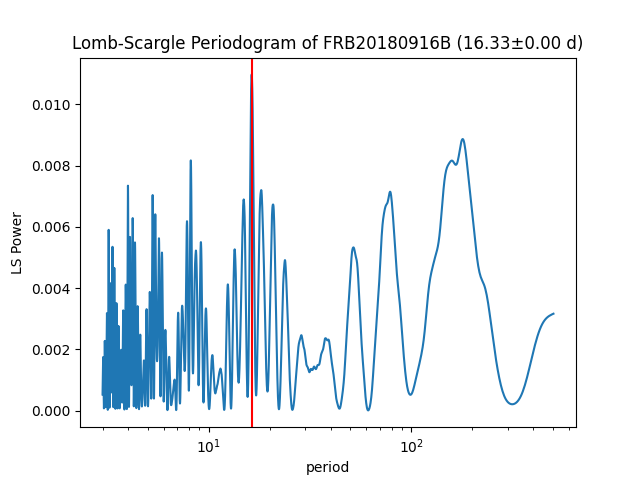
\includegraphics[width=0.3\textwidth,height=\textheight]{./img/FRB20180916B-periodogram-LS.png}
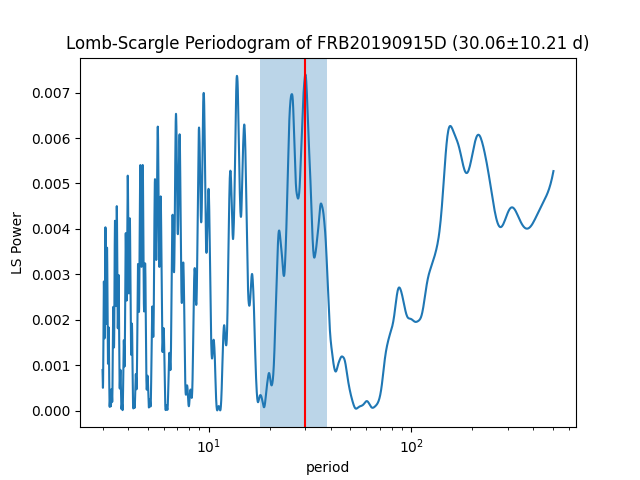
\includegraphics[width=0.3\textwidth,height=\textheight]{./img/FRB20190915D-periodogram-LS.png}
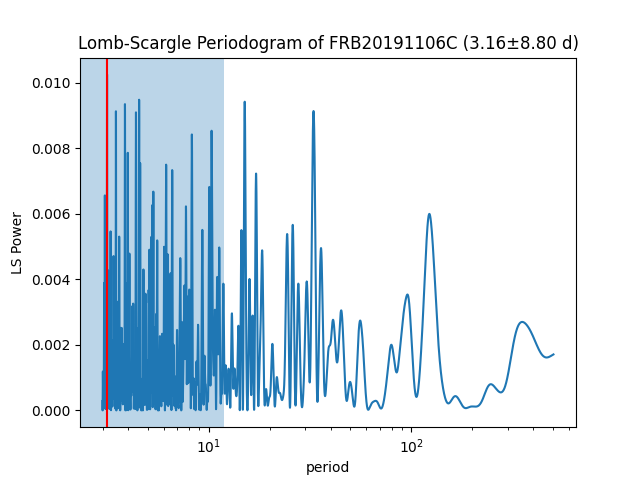
\includegraphics[width=0.3\textwidth,height=\textheight]{./img/FRB20191106C-periodogram-LS.png}
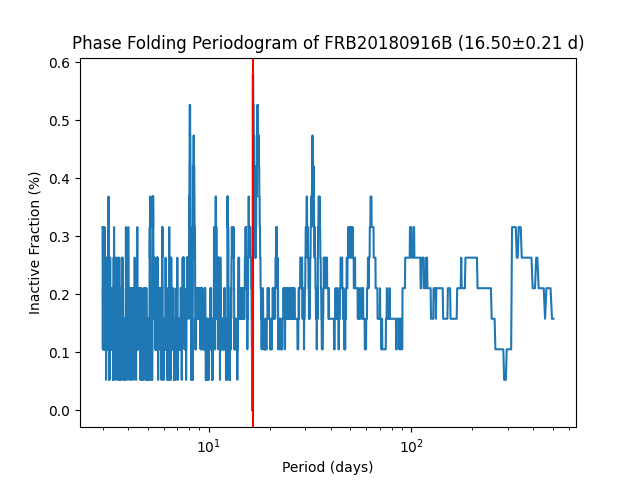
\includegraphics[width=0.3\textwidth,height=\textheight]{./img/FRB20180916B-periodogram-PF.png}
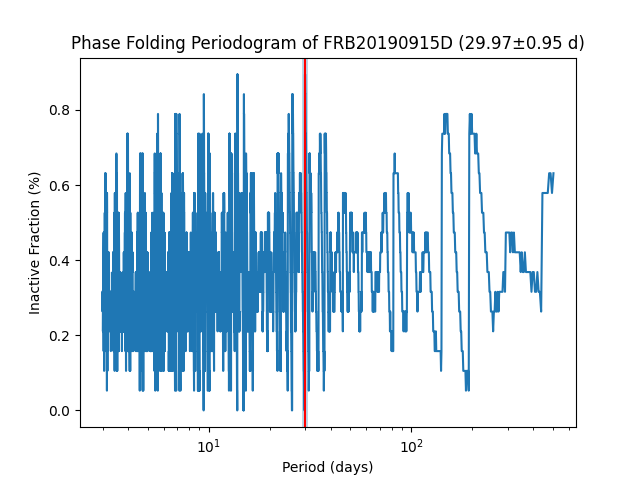
\includegraphics[width=0.3\textwidth,height=\textheight]{./img/FRB20190915D-periodogram-PF.png}
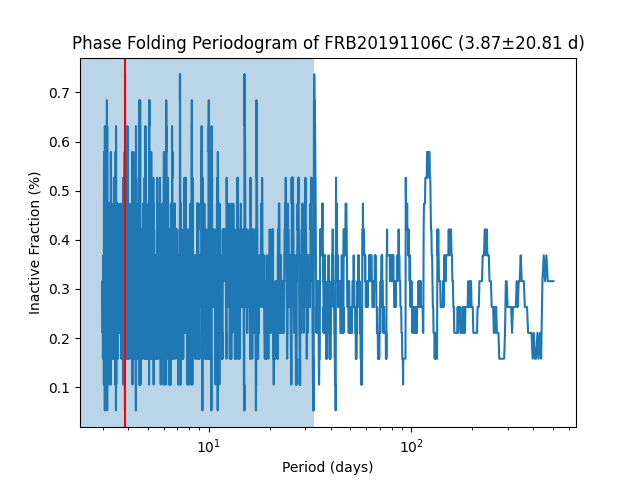
\includegraphics[width=0.3\textwidth,height=\textheight]{./img/FRB20191106C-periodogram-PF.png}
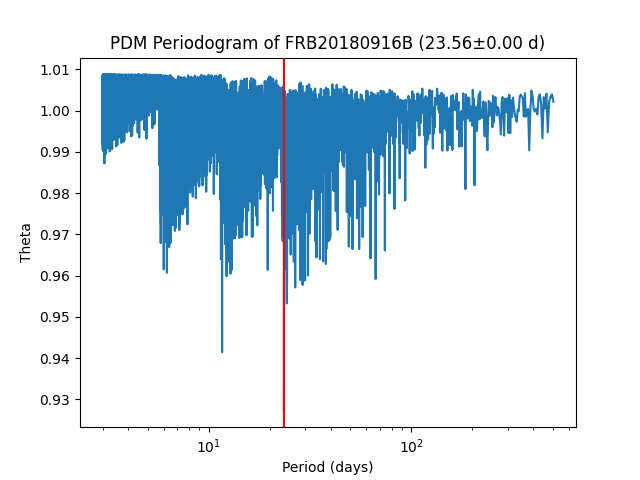
\includegraphics[width=0.3\textwidth,height=\textheight]{./img/FRB20180916B-periodogram-PDM.png}
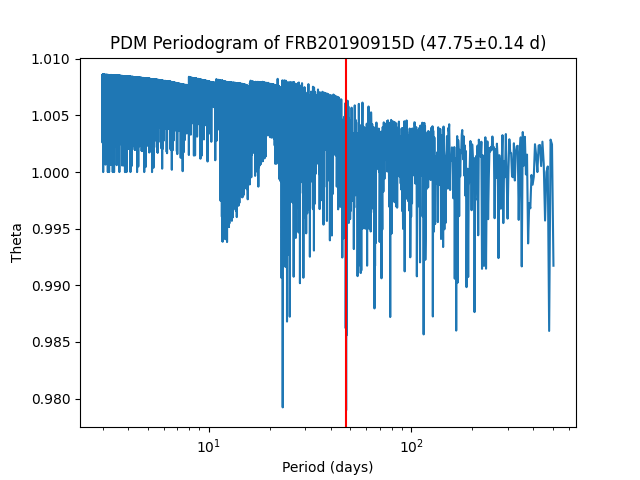
\includegraphics[width=0.3\textwidth,height=\textheight]{./img/FRB20190915D-periodogram-PDM.png}
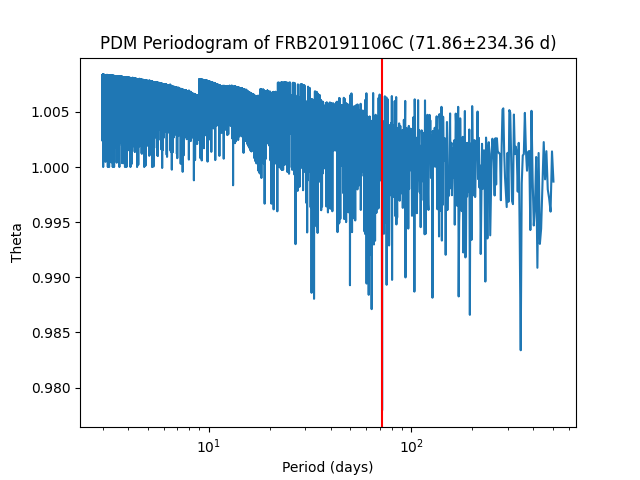
\includegraphics[width=0.3\textwidth,height=\textheight]{./img/FRB20191106C-periodogram-PDM.png}

}

\end{minipage}%

\caption{\label{fig-periodogram}The periodograms of FRB20180916B (left),
FRB20190915D (middle column) and FRB20191106C (right) using
Lomb--Scargle method (top), Duty Cycle method (middle row) and Phase
Dispersion Minimization (bottom).}

\end{figure}

\hypertarget{tbl-result}{}
\begin{longtable}[]{@{}lccc@{}}
\caption{\label{tbl-result}The periods obtained from the specified
methods in days and its uncertainty. The percentage in brackets for the
`Duty Cycle' column is the active fraction of the cycle.}\tabularnewline
\toprule\noalign{}
burst name & LS & DC & PDM \\
\midrule\noalign{}
\endfirsthead
\toprule\noalign{}
burst name & LS & DC & PDM \\
\midrule\noalign{}
\endhead
\bottomrule\noalign{}
\endlastfoot
FRB20180916B & 16.33±0.00 & 16.30±0.21 (36.8\%) & 23.56±0.00 \\
FRB20190915D & 30.06±10.21 & 29.97±0.95 (10.5\%) & 47.75±0.14 \\
FRB20191106C & 3.16±8.80 & 3.87±20.81 (26.3\%) & 71.86±234.36 \\
\end{longtable}

The results shown in Table~\ref{tbl-result} accompanied by
Figure~\ref{fig-periodogram} for FRB20180916B using Lomb--Scargle and
Duty Cycle methods are consistent with the periodicities from The
CHIME/FRB Collaboration et al. (2020) of 16.35±0.15 days and Sand et al.
(2023) of 16.34±0.07 days. This consistency indicates that the
methodology is reliable in determining periodicity using the available
data. The Phase Dispersion Minimization method, however, offshoots by
about \textasciitilde1.4 times the obtained periodicity from the
previous two methods.

This pattern also emerges in the results for FRB20190915D with
Lomb--Scargle and Duty Cycle methods showing a periodicity of
30.06±10.21 days and 29.97±0.95 days respectively, with Phase Dispersion
Minimization offshooting to 1.5\textasciitilde1.6 times the two values.
This hints that these values might point to the real periodicity of the
newly discovered FRB20190915D even though the available data is limited.
The Phase Dispersion Minimization seems to consistently obtain 1.5
\times period days which is somewhat like a harmonic, equivalent to the
second harmonic equivalent to \(1.5\times \lambda\) standing wave.

The same could not be said for FRB20191106C for two reasons. First,
although it has consistent values for the first two methods, the Phase
Dispersion Minimzation period is 18.5\textasciitilde22.7 times the
previous two values. This does not follow the pattern of the previous
FRBs. Secondly, we have to be careful in interpreting periodogram
values. While it is true that the first two values are consistent, it is
imperative to understand that 3 days is the minimum period chosen for
this analysis and periodograms tend to spike at high frequency limit,
which explains the high uncertainty.

\begin{figure}

\begin{minipage}[t]{0.33\linewidth}

{\centering 

\raisebox{-\height}{

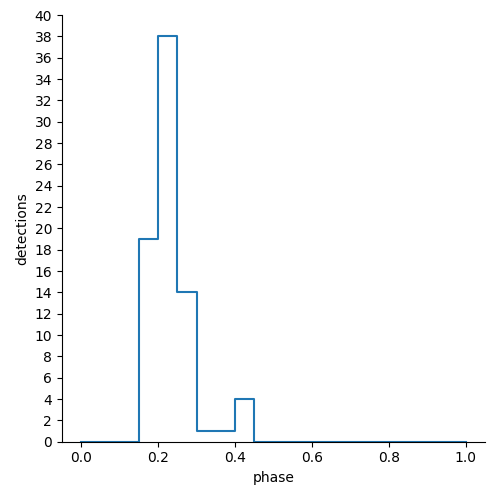
\includegraphics{./FRB20180916B-phase-16.33.png}

}

}

\subcaption{\label{fig-fold-FRB20180916B}FRB20180916B at 16.33 days}
\end{minipage}%
%
\begin{minipage}[t]{0.33\linewidth}

{\centering 

\raisebox{-\height}{

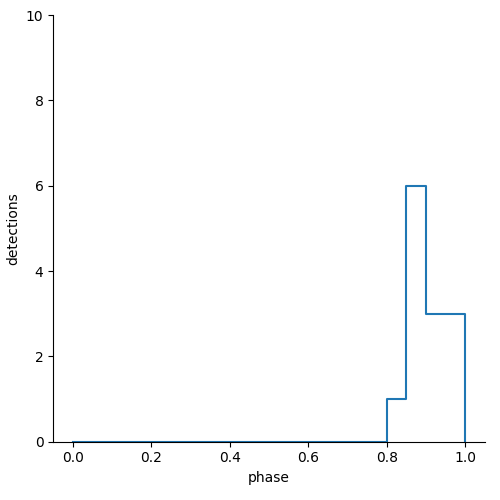
\includegraphics{./FRB20190915D-phase-30.06.png}

}

}

\subcaption{\label{fig-fold-FRB20190915D}FRB20190915D at 30.06 days}
\end{minipage}%
%
\begin{minipage}[t]{0.33\linewidth}

{\centering 

\raisebox{-\height}{

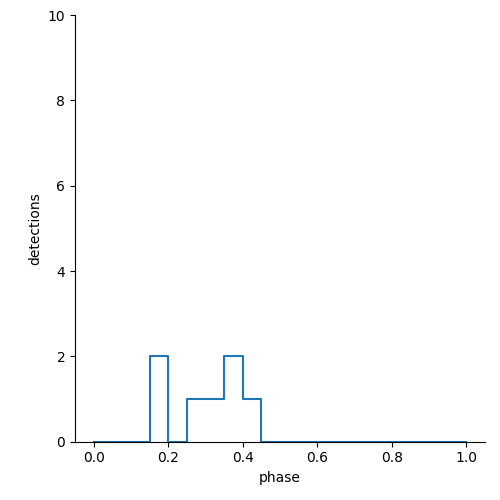
\includegraphics{./FRB20191106C-phase-3.16.png}

}

}

\subcaption{\label{fig-fold-FRB20191106C}FRB20191106C at 3.16 days}
\end{minipage}%

\caption{\label{fig-fold}Phase folded detection count of FRB at their
selected periods.}

\end{figure}

\hypertarget{discussion}{%
\section{Discussion}\label{discussion}}

\hypertarget{false-alarm-probability}{%
\subsection{False Alarm Probability}\label{false-alarm-probability}}

It is useful to quantify the false alarm probability (FAP) as a proxy of
confidence. The FAP is computed using the `bootstrap' method implemented
in astropy's \texttt{LombScargle} class. It is found that each FRBs has
a FAP of 13.3\% (FRB20180916B), 57.0\% (FRB20190915D) and 66.0\%
(FRB20191106C). These values are consistent with the heuristics in the
preceding paragraphs that the value for FRB20180916B has a higher
confidence than for FRB20190915D while values obtained for FRB20191106C
has the least confidence. The fact that the FAP for FRB20190915D is
slightly above 50\% but not any higher might be due to the fact that its
detection only happens in a small time frame compared to the observation
window. Fixing the window to be between 20 Jun 2019 and 15 May 2020
reduces the FAP to 44.2\% -- suggesting that there is more than 50\%
confidence that it has a periodicity if treated as a time-limited event.
Further discussion on this property is in Section~\ref{sec-why-30}.

\hypertarget{waiting-time-distribution}{%
\subsection{Waiting time distribution}\label{waiting-time-distribution}}

One might wonder what distinguishes FRB20190915D from FRB20191106C which
allowed one to have periodicity despite limited samples? Looking at the
waiting time distribution in Figure~\ref{fig-waitingtime}, FRB20190915D
clearly shows bimodal distribution consistent with FRB20180916B (shown
here) and FRB20121102A (shown in Hewitt et al. (2022) and Jahns et al.
(2022)). Additionally, the waiting time of FRB20191106C is concentrated
in the longer timescale compared to the bimodal distribution. It seems
that a bimodal distribution is required for an FRB to have a
well-defined periodicity.

\begin{figure}

{\centering 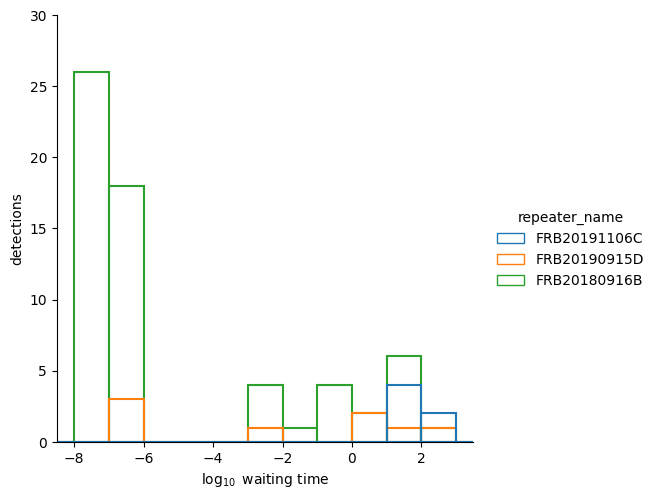
\includegraphics{./img/waiting.png}

}

\caption{\label{fig-waitingtime}The waiting time distribution of
FRB20191106C, FRB20191106C, and FRB20190916B in the \(\log_{10}\)
scale.}

\end{figure}

\hypertarget{sec-why-30}{%
\subsection{Where is the rest of the detections?}\label{sec-why-30}}

If it is indeed that FRB20190915D has a 30 day periodicity, why is there
no additional detections within the 3 year window of the catalogue? It
might be the case that this FRB has a multi-term periodicity with this
value representing it's short-term periodicity. If that is the case,
it's long-term periodicity is expected to be more than 2 years which is
yet to be seen. However, this is the same as hypothesizing that
repeaters are possible repeaters with not-yet-observed repetition.

Another hypothesis that might explain this seemingly lack of regular
detection is that FRB20190915D is a cataclysmic event with a periodic
pulse and stopping at a certain point, such as the inspiraling of two
magnetic bodies whose interaction releases some radio bursts. This might
explain the ever increasing detection count as it reaches peak and then
no longer bursting.

\begin{figure}

{\centering 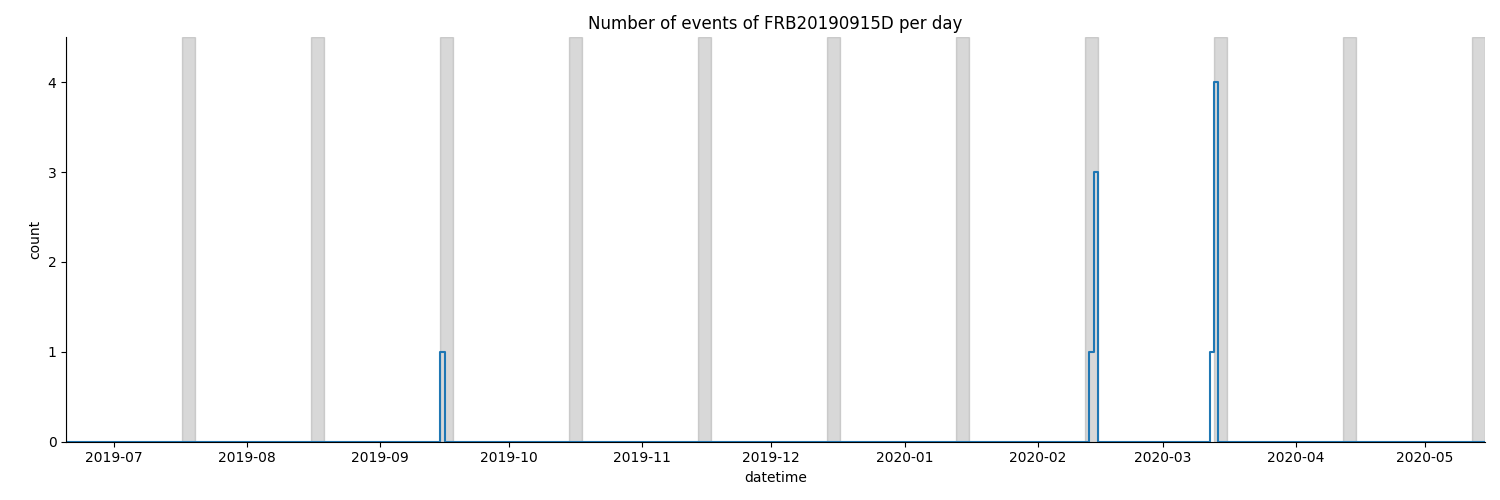
\includegraphics{./img/FRB20190915D-countplot.png}

}

\caption{\label{fig-FRB20190915D-countplot}The number of detections per
day of FRB20190915D between 20th Jun 2019 between 15th May 2020. The
gray coloured regions indicate the active fractions (10\%) in a 30 day
cycle from 25th Jul 2018. Note that this graph focuses on this small
timeframe because the datasets spans from 25th Jul 2018 to 26th Apr 2021
but is empty throughout the beginning and end for the specified FRB.}

\end{figure}

\hypertarget{conclusion}{%
\section{Conclusion}\label{conclusion}}

This paper determines that it is possible to evaluate the periodicity of
FRBs despite small event counts. The choice of periodogram seems to
matter as the Phase Dispersion Minimization method seems to offshoot for
FRBs, but using multiple periodogram methods help find a consistent
pattern. The bimodal distribution of waiting times seems crucial in the
determinability of its periodicity. This paper also hints that there
might a new class of FRB whose repeatability seems limited -- such as an
inspiraling collision -- suggesting that FRBs might be divided into
three classes: (i) continuously repeating, (ii) limited repeating, or
(iii) one-off.

\hypertarget{acknowledgement}{%
\section{Acknowledgement}\label{acknowledgement}}

The authors wishes to thank the team from CHIME/FRB for their initiative
in open data which allowed this work to happen. We would like to
acknowledge the grant \textless TODO: GRANT NUMBER\textgreater{} for
funding the research activities of the radio cosmology lab group in
Universiti Malaya in which the development of the Malaysian VGOS radio
telescope is taking place.

\hypertarget{references}{%
\section*{References}\label{references}}
\addcontentsline{toc}{section}{References}

\hypertarget{refs}{}
\begin{CSLReferences}{1}{0}
\leavevmode\vadjust pre{\hypertarget{ref-andersen_CHIMEFRBDiscovery_2023}{}}%
Andersen, B. C., K. Bandura, M. Bhardwaj, P. J. Boyle, C. Brar, T.
Cassanelli, S. Chatterjee, et al. 2023. {``{CHIME}/{FRB Discovery} of 25
{Repeating Fast Radio Burst Sources}.''} \emph{The Astrophysical
Journal} 947 (January): 83.
\url{https://doi.org/10.3847/1538-4357/acc6c1}.

\leavevmode\vadjust pre{\hypertarget{ref-bannister_SingleFastRadio_2019}{}}%
Bannister, K. W., A. T. Deller, C. Phillips, J. -P. Macquart, J. X.
Prochaska, N. Tejos, S. D. Ryder, et al. 2019. {``A Single Fast Radio
Burst Localized to a Massive Galaxy at Cosmological Distance.''}
\emph{Science} 365 (August): 565--70.
\url{https://doi.org/10.1126/science.aaw5903}.

\leavevmode\vadjust pre{\hypertarget{ref-bohanchen_UncloakingHiddenRepeating_2021}{}}%
Bo Han Chen, Tetsuya Hashimoto, Tomotsugu Goto, Seong Jin Kim, Daryl Joe
D. Santos, Alvina Y. L. On, Ting-Yi Lu, and Tiger Y. -Y. Hsiao. 2021.
{``Uncloaking Hidden Repeating Fast Radio Bursts with Unsupervised
Machine Learning.''} \emph{Monthly Notices of the Royal Astronomical
Society} 509 (1): 1227--36.
\url{https://doi.org/10.1093/mnras/stab2994}.

\leavevmode\vadjust pre{\hypertarget{ref-chatterjee_DirectLocalizationFast_2017}{}}%
Chatterjee, S., C. J. Law, R. S. Wharton, S. Burke-Spolaor, J. W. T.
Hessels, G. C. Bower, J. M. Cordes, et al. 2017. {``A Direct
Localization of a Fast Radio Burst and Its Host.''} \emph{Nature} 541
(January): 58--61. \url{https://doi.org/10.1038/nature20797}.

\leavevmode\vadjust pre{\hypertarget{ref-chen_OneoffRepeatingFast_2022}{}}%
Chen, Hao-Yan, Wei-Min Gu, Mouyuan Sun, and Tuan Yi. 2022. {``One-Off
and {Repeating Fast Radio Bursts}: {A Statistical Analysis}.''}
\emph{The Astrophysical Journal} 939 (November): 27.
\url{https://doi.org/10.3847/1538-4357/ac958a}.

\leavevmode\vadjust pre{\hypertarget{ref-cui_FastRadioBursts_2021}{}}%
Cui, Xiang-Han, Cheng-Min Zhang, Shuang-Qiang Wang, Jian-Wei Zhang, Di
Li, Bo Peng, Wei-Wei Zhu, Na Wang, et al. 2021. {``Fast Radio Bursts: Do
Repeaters and Non-Repeaters Originate in Statistically Similar
Ensembles?''} \emph{Monthly Notices of the Royal Astronomical Society}
500 (January): 3275--80. \url{https://doi.org/10.1093/mnras/staa3351}.

\leavevmode\vadjust pre{\hypertarget{ref-cui_StatisticalPropertiesFast_2021}{}}%
Cui, Xiang-Han, Cheng-Min Zhang, Shuang-Qiang Wang, Jian-Wei Zhang, Di
Li, Bo Peng, Wei-Wei Zhu, Richard Strom, et al. 2021. {``Statistical
Properties of Fast Radio Bursts Elucidate Their Origins: Magnetars Are
Favored over Gamma-Ray Bursts.''} \emph{Research in Astronomy and
Astrophysics} 21 (8): 211.
\url{https://doi.org/10.1088/1674-4527/21/8/211}.

\leavevmode\vadjust pre{\hypertarget{ref-hewitt_AreciboObservationsBurst_2022}{}}%
Hewitt, D. M., M. P. Snelders, J. W. T. Hessels, K. Nimmo, J. N. Jahns,
L. G. Spitler, K. Gourdji, et al. 2022. {``Arecibo Observations of a
Burst Storm from {FRB 20121102A} in 2016.''} \emph{Monthly Notices of
the Royal Astronomical Society} 515 (September): 3577--96.
\url{https://doi.org/10.1093/mnras/stac1960}.

\leavevmode\vadjust pre{\hypertarget{ref-jahns_FRB20121102ANovember_2022}{}}%
Jahns, J. N., L. G. Spitler, K. Nimmo, D. M. Hewitt, M. P. Snelders, A.
Seymour, J. W. T. Hessels, K. Gourdji, D. Michilli, and G. H.
Hilmarsson. 2022. {``The {FRB 20121102A November} Rain in 2018 Observed
with the {Arecibo Telescope}.''} \emph{Monthly Notices of the Royal
Astronomical Society} 519 (November): 666--87.
\url{https://doi.org/10.1093/mnras/stac3446}.

\leavevmode\vadjust pre{\hypertarget{ref-katz_AbsencePeriodicityRepeating_2022}{}}%
Katz, J. I. 2022. {``The Absence of Periodicity in Repeating {FRB}.''}
\emph{Monthly Notices of the Royal Astronomical Society} 513 (June):
1925--31. \url{https://doi.org/10.1093/mnras/stac1059}.

\leavevmode\vadjust pre{\hypertarget{ref-lin_BURSTTBustlingUniverse_2022}{}}%
Lin, Hsiu-Hsien, Kai-yang Lin, Chao-Te Li, Yao-Huan Tseng, Homin Jiang,
Jen-Hung Wang, Jen-Chieh Cheng, et al. 2022. {``{BURSTT}: {Bustling
Universe Radio Survey Telescope} in {Taiwan}.''} \emph{Publications of
the Astronomical Society of the Pacific} 134 (September): 094106.
\url{https://doi.org/10.1088/1538-3873/ac8f71}.

\leavevmode\vadjust pre{\hypertarget{ref-lomb_LeastSquaresFrequencyAnalysis_1976}{}}%
Lomb, N. R. 1976. {``Least-{Squares Frequency Analysis} of {Unequally
Spaced Data}.''} \emph{Astrophysics and Space Science} 39 (February):
447--62. \url{https://doi.org/10.1007/BF00648343}.

\leavevmode\vadjust pre{\hypertarget{ref-lorimer_BrightMillisecondRadio_2007}{}}%
Lorimer, D. R., M. Bailes, M. A. McLaughlin, D. J. Narkevic, and F.
Crawford. 2007. {``A Bright Millisecond Radio Burst of Extragalactic
Origin.''} \emph{Science} 318 (5851): 777--80.
\url{https://doi.org/10.1126/science.1147532}.

\leavevmode\vadjust pre{\hypertarget{ref-luo_MachineLearningClassification_2022}{}}%
Luo, Jia-Wei, Jia-Ming Zhu-Ge, and Bing Zhang. 2022. {``Machine
{Learning Classification} of {CHIME} Fast Radio Bursts: {I}. {Supervised
Methods}.''} \emph{Monthly Notices of the Royal Astronomical Society},
November, stac3206. \url{https://doi.org/10.1093/mnras/stac3206}.

\leavevmode\vadjust pre{\hypertarget{ref-petroff_FastRadioBursts_2019}{}}%
Petroff, E., J. W. T. Hessels, and D. R. Lorimer. 2019. {``Fast Radio
Bursts.''} \emph{The Astronomy and Astrophysics Review} 27 (1): 75.
\url{https://doi.org/10.1007/s00159-019-0116-6}.

\leavevmode\vadjust pre{\hypertarget{ref-petroff_FastRadioBursts_2022}{}}%
---------. 2022. {``Fast Radio Bursts at the Dawn of the 2020s.''}
\emph{The Astronomy and Astrophysics Review} 30 (1): 49.
\url{https://doi.org/10.1007/s00159-022-00139-w}.

\leavevmode\vadjust pre{\hypertarget{ref-platts_LivingTheoryCatalogue_2019}{}}%
Platts, E., A. Weltman, A. Walters, S. P. Tendulkar, J. E. B. Gordin,
and S. Kandhai. 2019. {``A {Living Theory Catalogue} for {Fast Radio
Bursts}.''} \emph{Physics Reports} 821 (August): 1--27.
\url{https://doi.org/10.1016/j.physrep.2019.06.003}.

\leavevmode\vadjust pre{\hypertarget{ref-pleunis_FastRadioBurst_2021}{}}%
Pleunis, Ziggy, Deborah C. Good, Victoria M. Kaspi, Ryan Mckinven, Scott
M. Ransom, Paul Scholz, Kevin Bandura, et al. 2021. {``Fast {Radio Burst
Morphology} in the {First CHIME}/{FRB Catalog}.''} \emph{The
Astrophysical Journal} 923 (1): 1.
\url{https://doi.org/10.3847/1538-4357/ac33ac}.

\leavevmode\vadjust pre{\hypertarget{ref-rajwade_PossiblePeriodicActivity_2020}{}}%
Rajwade, K M, M B Mickaliger, B W Stappers, V Morello, D Agarwal, C G
Bassa, R P Breton, et al. 2020. {``Possible Periodic Activity in the
Repeating {FRB} 121102.''} \emph{Monthly Notices of the Royal
Astronomical Society} 495 (4): 3551--58.
\url{https://doi.org/10.1093/mnras/staa1237}.

\leavevmode\vadjust pre{\hypertarget{ref-ravi_FastRadioBurst_2019}{}}%
Ravi, V., M. Catha, L. D'Addario, S. G. Djorgovski, G. Hallinan, R.
Hobbs, J. Kocz, et al. 2019. {``A Fast Radio Burst Localized to a
Massive Galaxy.''} \emph{Nature} 572 (August): 352--54.
\url{https://doi.org/10.1038/s41586-019-1389-7}.

\leavevmode\vadjust pre{\hypertarget{ref-sand_CHIMEFRBStudy_2023}{}}%
Sand, Ketan R., Daniela Breitman, Daniele Michilli, Victoria M. Kaspi,
Pragya Chawla, Emmanuel Fonseca, Ryan Mckinven, et al. 2023. {``A
{CHIME}/{FRB} Study of Burst Rate and Morphological Evolution of the
Periodically Repeating {FRB 20180916B}.''} \emph{arXiv e-Prints}.
\url{https://doi.org/10.48550/arXiv.2307.05839}.

\leavevmode\vadjust pre{\hypertarget{ref-scargle_StudiesAstronomicalTime_1982}{}}%
Scargle, J. D. 1982. {``Studies in Astronomical Time Series Analysis.
{II}. {Statistical} Aspects of Spectral Analysis of Unevenly Spaced
Data.''} \emph{The Astrophysical Journal} 263 (December): 835--53.
\url{https://doi.org/10.1086/160554}.

\leavevmode\vadjust pre{\hypertarget{ref-stellingwerf_PeriodDeterminationUsing_1978}{}}%
Stellingwerf, R. F. 1978. {``Period Determination Using Phase Dispersion
Minimization.''} \emph{The Astrophysical Journal} 224 (September):
953--60. \url{https://doi.org/10.1086/156444}.

\leavevmode\vadjust pre{\hypertarget{ref-thechimefrbcollaborationFirstCHIMEFRB2021}{}}%
The CHIME/FRB Collaboration, Mandana Amiri, Bridget C. Andersen, Kevin
Bandura, Sabrina Berger, Mohit Bhardwaj, Michelle M. Boyce, et al. 2021.
{``The {First CHIME}/{FRB Fast Radio Burst Catalog}.''} \emph{The
Astrophysical Journal Supplement Series} 257 (2): 59.
\url{https://doi.org/10.3847/1538-4365/ac33ab}.

\leavevmode\vadjust pre{\hypertarget{ref-thechimefrbcollaborationPeriodicActivityFast2020}{}}%
The CHIME/FRB Collaboration, M. Amiri, B. C. Andersen, K. M. Bandura, M.
Bhardwaj, P. J. Boyle, C. Brar, et al. 2020. {``Periodic Activity from a
Fast Radio Burst Source.''} \emph{Nature} 582 (7812): 351--55.
\url{https://doi.org/10.1038/s41586-020-2398-2}.

\leavevmode\vadjust pre{\hypertarget{ref-thechimefrbcollaborationCHIMEFastRadio2018}{}}%
The CHIME/FRB Collaboration, M. Amiri, K. Bandura, P. Berger, M.
Bhardwaj, M. M. Boyce, P. J. Boyle, et al. 2018. {``The {CHIME Fast
Radio Burst Project}: {System Overview}.''} \emph{The Astrophysical
Journal} 863 (1): 48. \url{https://doi.org/10.3847/1538-4357/aad188}.

\leavevmode\vadjust pre{\hypertarget{ref-vanderplas_UnderstandingLombScargle_2018}{}}%
VanderPlas, Jacob T. 2018. {``Understanding the
{Lomb}\textendash{{Scargle Periodogram}}.''} \emph{The Astrophysical
Journal Supplement Series} 236 (1): 16.
\url{https://doi.org/10.3847/1538-4365/aab766}.

\leavevmode\vadjust pre{\hypertarget{ref-zhang_StatisticalSimilarityRepeating_2022}{}}%
Zhang, Kongjun, Longbiao Li, Zhibin Zhang, Qinmei Li, Juanjuan Luo, and
Min Jiang. 2022. {``The {Statistical Similarity} of {Repeating} and
{Non-Repeating Fast Radio Bursts}.''} \emph{Universe} 8 (7): 355.
\url{https://doi.org/10.3390/universe8070355}.

\leavevmode\vadjust pre{\hypertarget{ref-zhu-ge_MachineLearningClassification_2022}{}}%
Zhu-Ge, Jia-Ming, Jia-Wei Luo, and Bing Zhang. 2022. {``Machine
{Learning Classification} of {Fast Radio Bursts}: {II}. {Unsupervised
Methods}.''} {arXiv}. \url{https://doi.org/10.48550/arXiv.2210.02471}.

\end{CSLReferences}



\end{document}
